\newcommand{\mfem}{\textit{MFEM}\xspace}
\newcommand{\glvis}{\textit{GLVis}\xspace}

\section{La biblioteca de elementos finitos \mfem. Problemas de evolución. Sistemas de EDP}
\subsection{Instalación}
\label{sec:03:instalacion}

\mfem \url{https://mfem.org} es «una biblioteca C++ gratuita, liviana
y escalable para métodos de elementos finitos».  Entre sus
características, descritas en \url{https://mfem.org/features}:
elementos 2D y 3D en triángulos, cuadriláteros, hexaedros, etc., orden
alto, $H^1$--conformes o $L^2$--discontinuos, elementos isogeométricos
(NURBS)...  Como todas las herramientas que se describirán a
continuación \mfem tiene licencia libre.

Aunque, como se puede comprobar en la web
\url{https://mfem.org/building/} existen versiones precompiladas que
usan sistemas de paquetes como \textit{Spack}, optaremos por la
instalación manual a partir de la compilación del código fuente.
Esto será más complicado, pero una vez sepamos hacerlo tendremos una
versión de la biblioteca expresamente compilada para nuestro sistema
y, en el futuro, tendremos garantizado el disponer de la última
versión, siempre que descarguemos las fuentes y volvamos a compilar.

Para ello, empezamos por descargar y descomprimir en una carpeta de
nuestro ordenador el archivo\footnote{Este tipo de archivos, de tipo
  \textit{.tar} y comprimidos con \texttt{gzip}, se usan desde hace
  décadas en sistemas UNIX.}  \texttt{.tgz} de su web,
\url{https://mfem.org/}.
\begin{itemize}
\item Esta será la última versión ``estable'' disponible del \textbf{código fuente de MFEM}.
\item De forma alternativa, se puede descargar la última versión ``inestable''de Github
\end{itemize}


A continuación, seguiremos las instrucciones del archivo
\href{https://raw.githubusercontent.com/mfem/mfem/master/INSTALL}{\textit{INSTALL}},
disponible en la web o en la carpeta donde descomprimimos anteriormente el código.

Comenzaremos por compilar una \textbf{versión secuencial} de \mfem. Más
adelante, hablaremos de la versión paralela. Los prerequisitos son:
\begin{itemize}
\item Un compilador de C++11, por ejemplo GCC.
\item Se recomienda disponer de una instalación de la biblioteca
  \textit{\glvis} para la visualización interactiva de mallas y
  funciones definidas sobre ellas.
\end{itemize}

Para la compilación suponemos además que se dispone de
\begin{itemize}
\item \textit{Make}
\item \textit{CMake}
\end{itemize}

\begin{lstlisting}[language=sh]
$ mkdir build
$ cd build
$ cmake ..
$ make -j 4
\end{lstlisting}

\begin{itemize}
\item En lo anterior, \texttt{build} es el nombre del directorio que
  elijamos para la compilación y \texttt{4} es el número de hilos
  paralelos durante el proceso de compilación.

\item \textit{CMake} es una
  herramienta de generación de código. Se ocupa de estudiar la
  disponibilidad en nuestro ordenador de las bibliotecas y otras
  herramientas necesarias para la compilación y, con esta información,
  genera un fichero \texttt{Makefile}.

\item Este fichero contiene las órdenes efectivas para la compilación
  y es utilizado (en la línea 4) por \textit{Make}, entorno de más
  bajo nivel que \textit{CMake}, para realizar este proceso y generar
  el código binario de \mfem.
\end{itemize}

Cuando finaliza la compilación, podemos ejecutar un primer test para
ver que la \mfem funciona correctamente ejecutando:
\begin{lstlisting}[language=sh]
$ make check
\end{lstlisting}
Esta orden compila y ejecuta el
\href{https://github.com/mfem/mfem/blob/master/examples/ex1.cpp}{ejemplo
  1} de la documentación de \mfem (ver
\url{https://mfem.org/examples}), que resuelve un problema para el
operador Laplaciano con condiciones de contorno Dirichlet.
\begin{lstlisting}
$ make check
[  0%] Built target copy_data
[  0%] Built target exec_prerequisites
[ 97%] Built target mfem
[100%] Built target ex1
Test project /home/rrgalvan/src/mfem/mfem-4.2/build
    Start 4: ex1_ser
1/1 Test #4: ex1_ser ..........................   Passed    0.15 sec

100% tests passed, 0 tests failed out of 1

Total Test time (real) =   0.15 sec
[100%] Built target check
\end{lstlisting}


Cuando finaliza la compilación, tendremos en nuestro directorio el fichero binario que contiene la biblioteca \mfem (por ejemplo, en sistemas GNU/Linux, el fichero \verb|libmfem.a|.


\subsection{El visualizador \glvis}
\label{sec:glvis}

Antes de su instalación, debemos asegurarnos de tener instalados los
paquetes que \glvis necesita. Esto varía en función del sistema
operativo (ver \url{https://glvis.org/building}).
Por ejemplo, en sistemas GNU/Linux derivados de la distribución \textit{Debian}, como \textit{Ubuntu}:
\begin{lstlisting}[language=sh]
$ apt-get install libfontconfig1-dev libfreetype-dev libsdl2-dev libglew-dev libglm-dev libpng-dev
\end{lstlisting}

Una vez contamos con los paquetes necesarios, podemos compilar, por
ejemplo usando directamente \textit{Make}. Será necesario indicar (en
la variable \verb|MFEM_dir|), el directorio donde, previamente, hemos
realizado la instalación de \mfem.
\begin{lstlisting}[language=sh]
$ make MFEM_DIR=../mfem-4.2/build -j 4
\end{lstlisting}

En este momento, podemos ejecutar \glvis, que queda a la espera de que
\mfem (u otro programa) le envíe datos para ser visualizados:
\begin{lstlisting}
$ ./glvis

       _/_/_/  _/      _/      _/  _/
    _/        _/      _/      _/        _/_/_/
   _/  _/_/  _/      _/      _/  _/  _/_/
  _/    _/  _/        _/  _/    _/      _/_/
   _/_/_/  _/_/_/_/    _/      _/  _/_/_/

Waiting for data on port 19916 ...
\end{lstlisting}
% $

Para hacer una prueba, abrimos otra terminal\footnote{O, en la misma
  terminal, pasamos \glvis a modo \textit{background} (pulsamos
  \texttt{Control+Z} y tecleamos \texttt{bg}).}. A continuación, nos
situamos en la carpeta \texttt{build/examples} (asumiendo que
\texttt{build} es el directorio de compilación de \mfem) y ejecutamos el ejemplo 1. Se obtendrá una representación gráfica similar a la mostrada en la figura

\begin{figure}
  \centering
  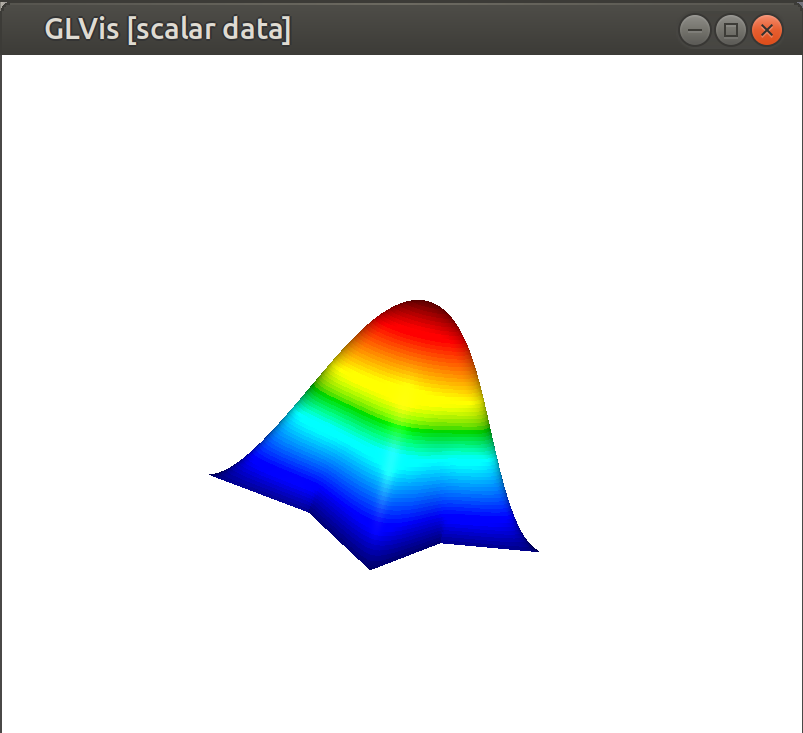
\includegraphics[width=0.3\linewidth]{img/ex1-glvis}
  \caption{Gráfica del ejemplo 1 de MFEM, visualizada con GLVis}
  \label{fig:ex1-glvis}
\end{figure}

Podemos modificar la visualización utilizando el ratón o alguna de las
combinaciones de tecla que se describen en el fichero
\href{https://raw.githubusercontent.com/glvis/glvis/master/README}{\textit{README}}. Por
ejemplo, podemos utilizar la tecla \texttt{m} para elegir la forma de
visualización de la malla, \texttt{S} para guardar\footnote{El fichero
  gráfico estará en el directorio desde donde se ejecutó el servidor
  de \glvis y su nombre será del tipo \texttt{GLVis\_s01.png}} una
captura de pantalla (\textit{snapshot}) y la tecla \texttt{q} para
salir (\textit{quit)}.


\subsection{Un primer ejemplo con \mfem}
\label{sec:3:un-primer-ejemplo}

\mfem se ha diseñado como una biblioteca C++ cuya jerarquía de clases
proporciona una serie de bloques básicos para desarrollar algoritmos
de tipo elementos finitos. Estos bloques básicos se describen
brevemente en \url{https://mfem.org/fem}. La jerarquía de clases se
describe por completo en la página web de
\href{https://mfem.github.io/doxygen/html/index.html}{documentación
  del código C++}\footnote{Esta página es generada automáticamente a
  partir de los comentarios incluidos en el código fuente, utilizando
  \href{https://www.doxygen.nl/index.html}{Doxygen}, una excelente
  herramienta para documentación en C++ (y otros lenguajes)} de \mfem.

Para comenzar a familiarizarse con la biblioteca \mfem, es
recomendable comenzar por el estudio de los ejemplos «canónicos»
disponibles en \url{https://mfem.org/examples/} y en el subdirectorio
\texttt{examples} del código fuente de \mfem.

Estudiaremos a continuación el
\href{https://github.com/mfem/mfem/blob/master/examples/ex1.cpp}{ejemplo
  1} de la documentación. Atendiendo a los comentarios insertados en
el código fuente, este ejemplo se divide en los siguientes apartados:
\begin{enumerate}
\item Analizar las «opciones», parámetros que pueden ser
  recibidos eventualmente desde la línea de comandos.
\item Habilitar, optativamente, dispositivos de hardware, como GPU, y
  modelos de programación, como CUDA u OpenMP.
\item Leer de un archivo la \textbf{malla} (formada por triángulos,
  cuadriláteros, hexaedros, ...).
\item Refinar (uniformemente) la malla hasta la resolución deseada.
\item Definir un \textbf{espacio de elementos finitos}.
\item Determinar la lista de nodos a los que se asociarán condiciones
  de contorno Dirichlet.
\item Configurar la \textbf{forma lineal} $b(\cdot)$ correspondiente al
  segundo miembro de la formulación variacional.
\item Definir una \textbf{función de elementos finitos} sobre la malla, $x$,
  que recogerá la solución.
\item Configurar la \textbf{forma bilineal}, $a(\cdot,\cdot)$, correspondiente
  a la formulación variacional, en este caso para el operador laplaciano.
\item \textbf{Montar el sistema de ecuaciones} lineales, añadiendo
  transformaciones como eliminación de condiciones de contorno
  esenciales (Dirichlet). Aquí (o previamente) se incluye el
  ensamblado de las formas bilineal y lineal en matriz $A$ y vector $B$.
\item \textbf{Resolver} el sistema de ecuaciones $A\, X= B$, obteniendo el vector $X$.
\item \textbf{Reconstruir la solución como función} de elementos finitos sobre la malla (en la variable $x$).
\item Grabar la malla y la solución para post-procesarla en el futuro.
\item Enviar la solución a \glvis para su visualización.
\item \textbf{Destruir} objetos para liberar memoria.
\end{enumerate}

%%% Local Variables:
%%% mode: latex
%%% TeX-master: "efavanzados.tex"
%%% End:
